
\subsection{Video en Youtube}
\begin{center}
\href{https://youtu.be/xjCqE8HniWs}{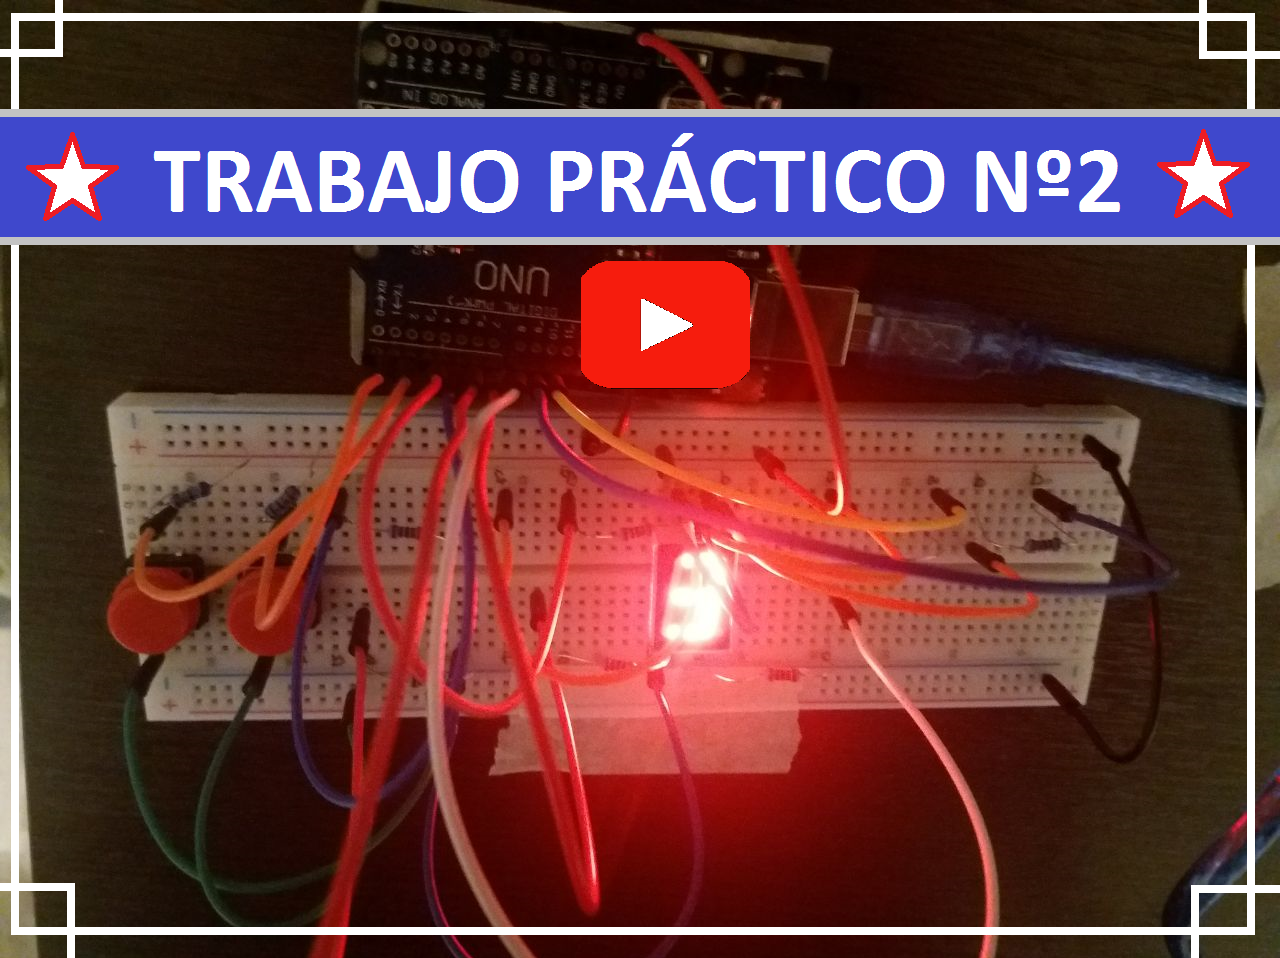
\includegraphics[width=.8\linewidth]{imagenes/VIDEO TP2.png}}
\end{center}

\subsection{Fotos}
\begin{center}

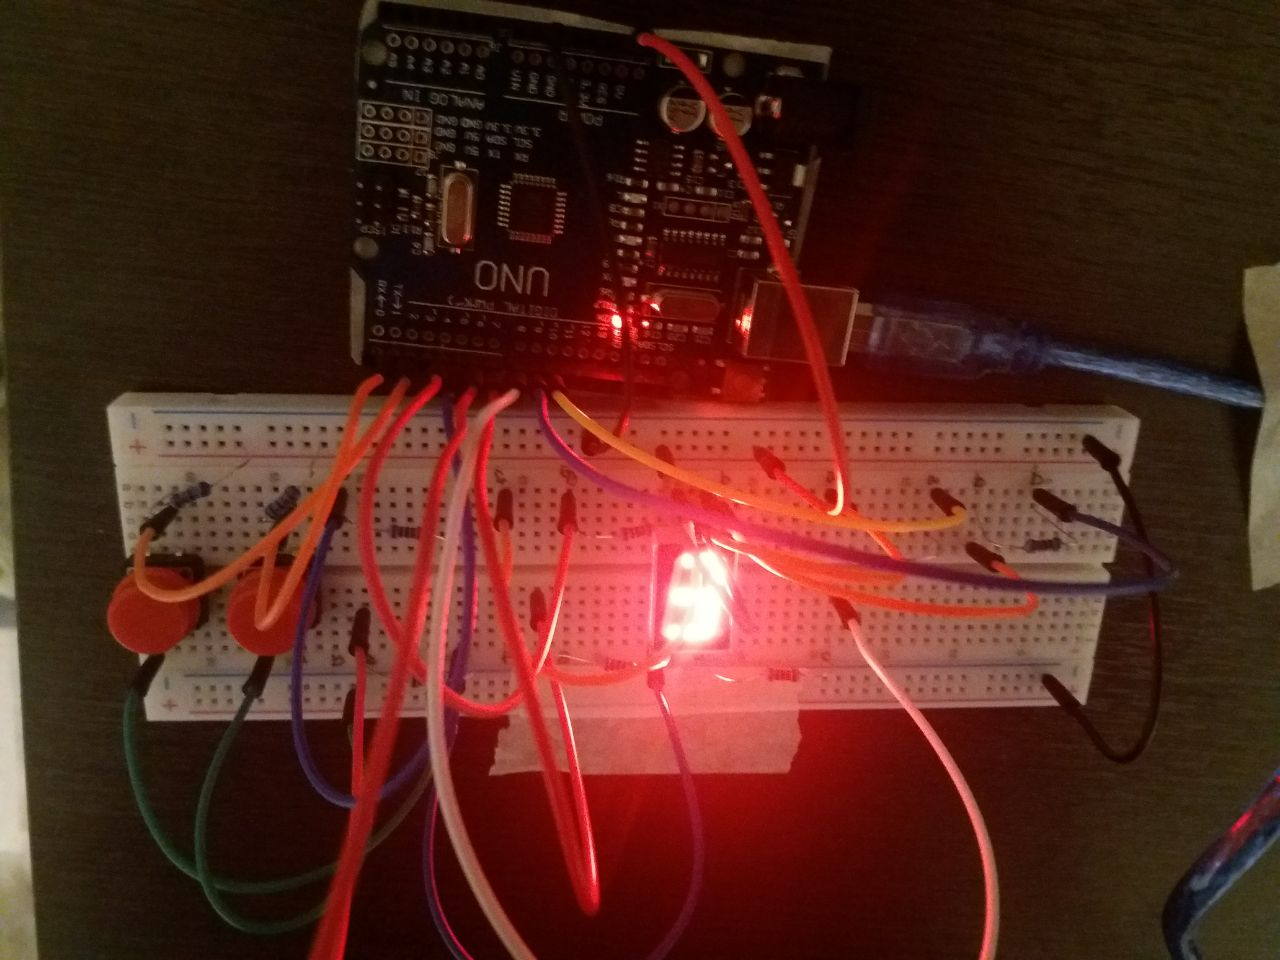
\includegraphics[width=.8\linewidth]{imagenes/photo5008481670650767804.jpg}

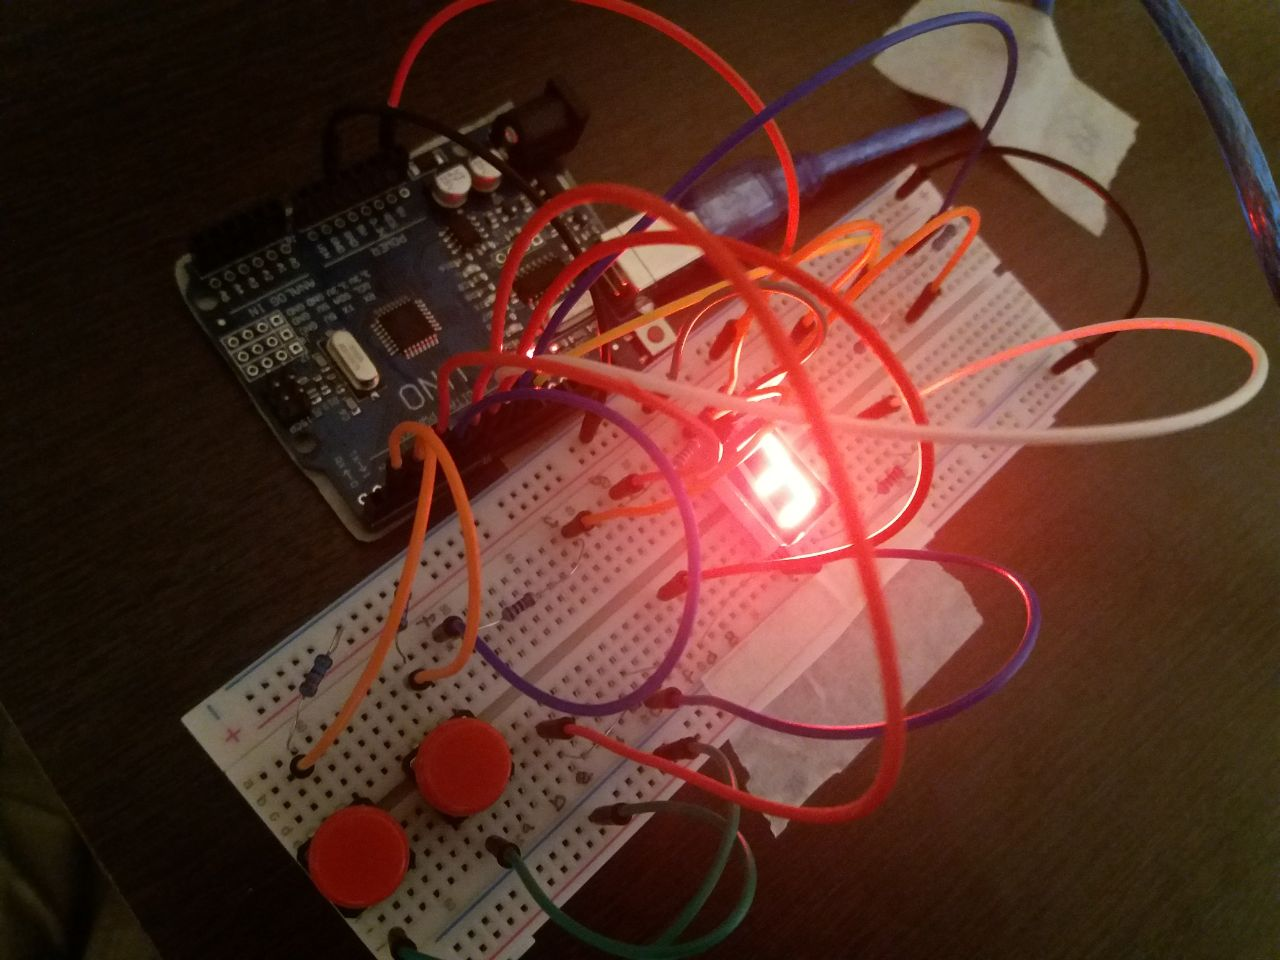
\includegraphics[width=.8\linewidth]{imagenes/photo5008481670650767805.jpg}

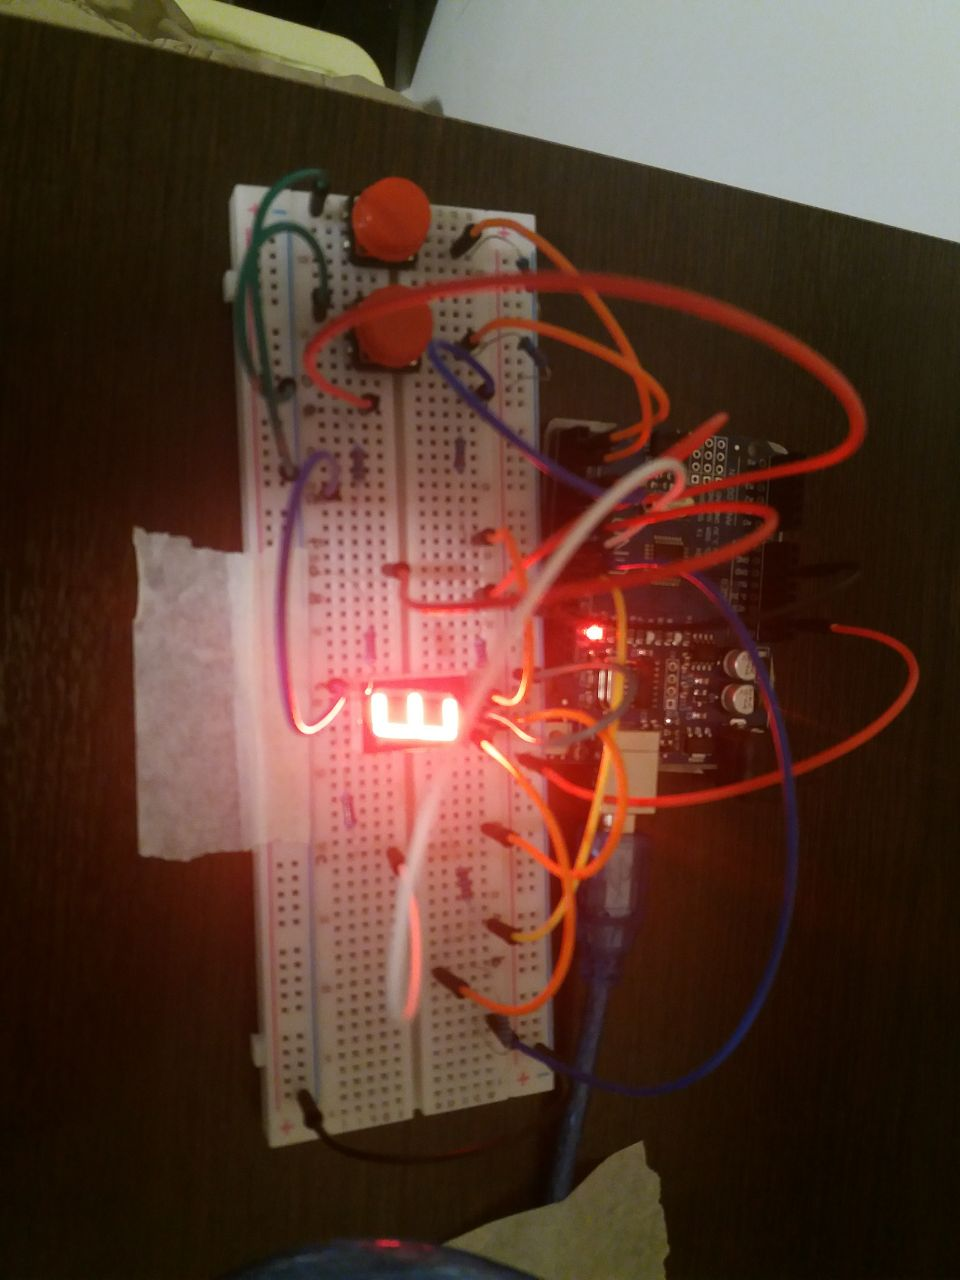
\includegraphics[width=\linewidth]{imagenes/photo5008481670650767806.jpg}
\end{center}


\section{Conclusiones}\label{sec:conclusion}

\begin{itemize}
    \item Se aprendió a usar DDR, PIN Y PORT
    \item Se aprendió a usar EICRA, EIMSK y CALL
    \item Se usó push y pop para evitar pisar variables que queremos preservar su valor
    \item Se vio que la rutina de delay puede ser muy útil de tener a mano para cualquier programa
    \item Se aprendió a leer un pin de un puerto, setear un valor de un puerto y poner como entrada  o salida.
    \item Se aplicaron los conceptos de interrupciones y de direccionamiento indirecto.
\end{itemize}

\section{Fuentes}

\begin{itemize}
    \item Datasheet de ATMega328P
    \item https://www.electricrcaircraftguy.com/2014/02/arduino-power-current-and-voltage.html
    \item https://aprendiendoarduino.wordpress.com/2016/11/09/alimentacion-arduino/
\end{itemize}